% questions.tex —— 1977 年·江苏苏州地区初试卷 · 题目内容片段（无答案）
% 由 tools/generate_projects.py 依来源总账自 1977/1977_数学真题_江苏苏州地区初试_试题.md 生成，勿手改（改源 MD 后重跑）


\gkpart{江苏苏州地区初试卷}

\begin{gktip}
\textbf{来源说明}：本卷为 1977 年高校招生苏州地区初试（预选）数学试卷，依据固定源 PDF 第 1—2 页逐题转录。源 PDF 为汇编材料扫描件，第 1 页页首印有分节标题「十二、苏州地区」，同页左下角印有原书页码 248，第 2 页无页码。原卷大题号用中文数字「一、二、三、四、五、六」，本库转写为「\textbf{N．}」；大题一、二、三的小题原卷用阿拉伯数字「1．2．…」编号，大题五的小题原卷已用「（1）（2）（3）」编号，本库统一转写为「（N）」（补齐括号后空格）。原卷末尾另有「附加题」两题，用阿拉伯数字「1．2．」编号，本库转写为「\textbf{附加题 N．}」，不计入正式题量。原卷无分值标注，大题四、六无小问。源卷为纯题面扫描，未附答案；配套答案与解析为本库编者独立推导，\textbf{非官方标准答案}。
\end{gktip}

\par\medskip

\begin{question}
\gkti{1}

（1） 化简：$(3y-1)^2-(3y-1)(3y+1)+3(y-1)$。

（2） 因式分解：$4x^4-y^4$。

（3） 计算：$(a+b-c)(a-b+c)$。

\Needspace{5\baselineskip}
（4） 计算：

\nopagebreak[4]
\[
\left(\frac{a-2b}{a+2b}-\frac{a+2b}{a-2b}\right)\div\frac{4ab}{4b^2c-a^2c}.
\]

\Needspace{5\baselineskip}
（5） 计算：

\nopagebreak[4]
\[
\sqrt[3]{1-\sqrt2}\cdot\sqrt[6]{3+2\sqrt2}-\frac1{1-\sqrt2}.
\]

\end{question}
\begin{question}
\gkti{2}

\Needspace{5\baselineskip}
（1） 解方程：

\nopagebreak[4]
\[
3+\frac{5x-1}{2}=x-\frac{1-3x}{5}.
\]

（2） 解方程：$x^2+x-2=0$。

\Needspace{5\baselineskip}
（3） 解方程组：

\nopagebreak[4]
\[
\begin{cases}
3x+2y-1=0\\
2x-3y+8=0
\end{cases}
\]

（4） 解不等式：$3(2y-5)+4\geqslant8y-7$。

\Needspace{0.4\textheight}
\end{question}
\begin{question}
\gkti{3}

（1） 计算：$4\sin30^\circ-3\operatorname{tg}45^\circ+2\cos30^\circ$。

（2） 在 $\triangle ABC$ 中，$C=90^\circ$，$a=2$，$b=1$，求 $\sin B$，$\operatorname{tg}A$。

（3） 在 $\triangle ABC$ 中，$M\text{、}N$ 分别是 $AB\text{、}AC$ 的中点，如果 $\triangle ABC$ 的面积是 $20$ 平方厘米，求 $\triangle AMN$ 的面积。

（4） 如图，$AB$ 为半圆的直径，$CD\perp AB$，求证：$CD^2=AD\cdot BD$。

\begin{gktip}
原源 PDF 第 1 页附有半圆、直径与垂线的示意图；LaTeX 版按源图重绘。
\end{gktip}
\nopagebreak[4]
\begin{center}% 1977 年江苏苏州地区初试卷第三题（4）小题：AB 为半圆的直径，CD⊥AB 于 D，C 在圆上（按源卷第1页布局）
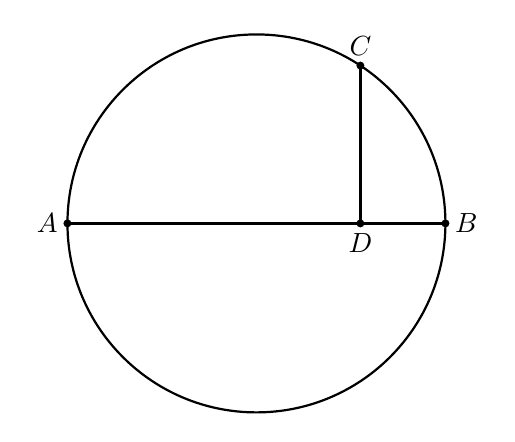
\begin{tikzpicture}[scale=1.2]
  \coordinate (O) at (0,0);
  \coordinate (A) at (-2,0);
  \coordinate (B) at (2,0);
  \coordinate (D) at (1.1,0);
  \coordinate (C) at (1.1,1.67);
  \draw[thick] (O) circle (2);
  \draw[thick] (A)--(B);
  \draw[thick] (C)--(D);
  \fill (A) circle (1.2pt) node[left] {$A$};
  \fill (B) circle (1.2pt) node[right] {$B$};
  \fill (C) circle (1.2pt) node[above] {$C$};
  \fill (D) circle (1.2pt) node[below] {$D$};
\end{tikzpicture}
\end{center}
\nopagebreak[4]
（5） 求 $P_1(0,-5)$ 和 $P_2(-1,2)$ 两点间的距离。

\end{question}
\begin{question}
\gkti{4}某机器厂第三季度共制造机器 $331$ 台，已知七月份制造 $100$ 台，求第三季度的月平均增长率。

\end{question}
\begin{question}
\gkti{5}在 $\triangle ABC$ 中，$A=45^\circ$，$AB+AC=10\ \mathrm{cm}$，

（1） 用公式法表示 $\triangle ABC$ 的面积 $(S)$ 与一边长 $AB\ (x)$ 之间的函数关系；

（2） $x$ 为何值时 $S$ 为最大；

（3） 求 $S$ 的最大值。

\end{question}
\begin{question}
\gkti{6}过点 $P(1,0)$ 作圆 $(x+1)^2+y^2=1$ 的切线，求切线方程。

\textbf{附加题 1．} 求所有被 $3$ 除余数为 $1$ 的两位数的和。

\textbf{附加题 2．} 求立方抛物线 $y=x^3$ 和直线 $y=1$、$x=0$ 所围成的图形的面积。

\begin{gktip}
提示：$1^3+2^3+3^3+\cdots+n^3=\left[\dfrac{n(n+1)}{2}\right]^2$。
\end{gktip}

\end{question}